\documentclass[
  12pt,
  openright,
  twoside,
  a4paper,
  english,
  brazil
]{abntex2}

\usepackage[T1]{fontenc}
\usepackage{indentfirst}
\usepackage{pdfpages}
\usepackage[alf]{abntex2cite}
\usepackage{booktabs}
\usepackage{pifont}

\setlength{\parindent}{1.3cm}

\titulo{Implementação de um front end para representação intermediária \textit{LLVM}}

\autor{Bernardo Ferrari Mendonça}
\local{Brasil}
\data{2019}
\orientador{Rafael de Santiago}
\coorientador{Evandro Chagas Ribeiro da Costa}
\instituicao{
  Universidade Federal de Santa Catarina
  \par
  Departamento de Informática e Estatística
  \par
  Ciência da Computação
}

\tipotrabalho{Trabalho de Conclusão de Curso de Graduação}

\preambulo{Proposta de monografia submetida ao Programa
de Graduação em Ciência da Computação
para a obtenção do Grau de Bacharel.}

\begin{document}
\pretextual{}
\hypersetup{pageanchor=false}
\imprimircapa{}
\hypersetup{pageanchor=true}
\imprimirfolhaderosto{}

\begin{folhadeaprovacao}
  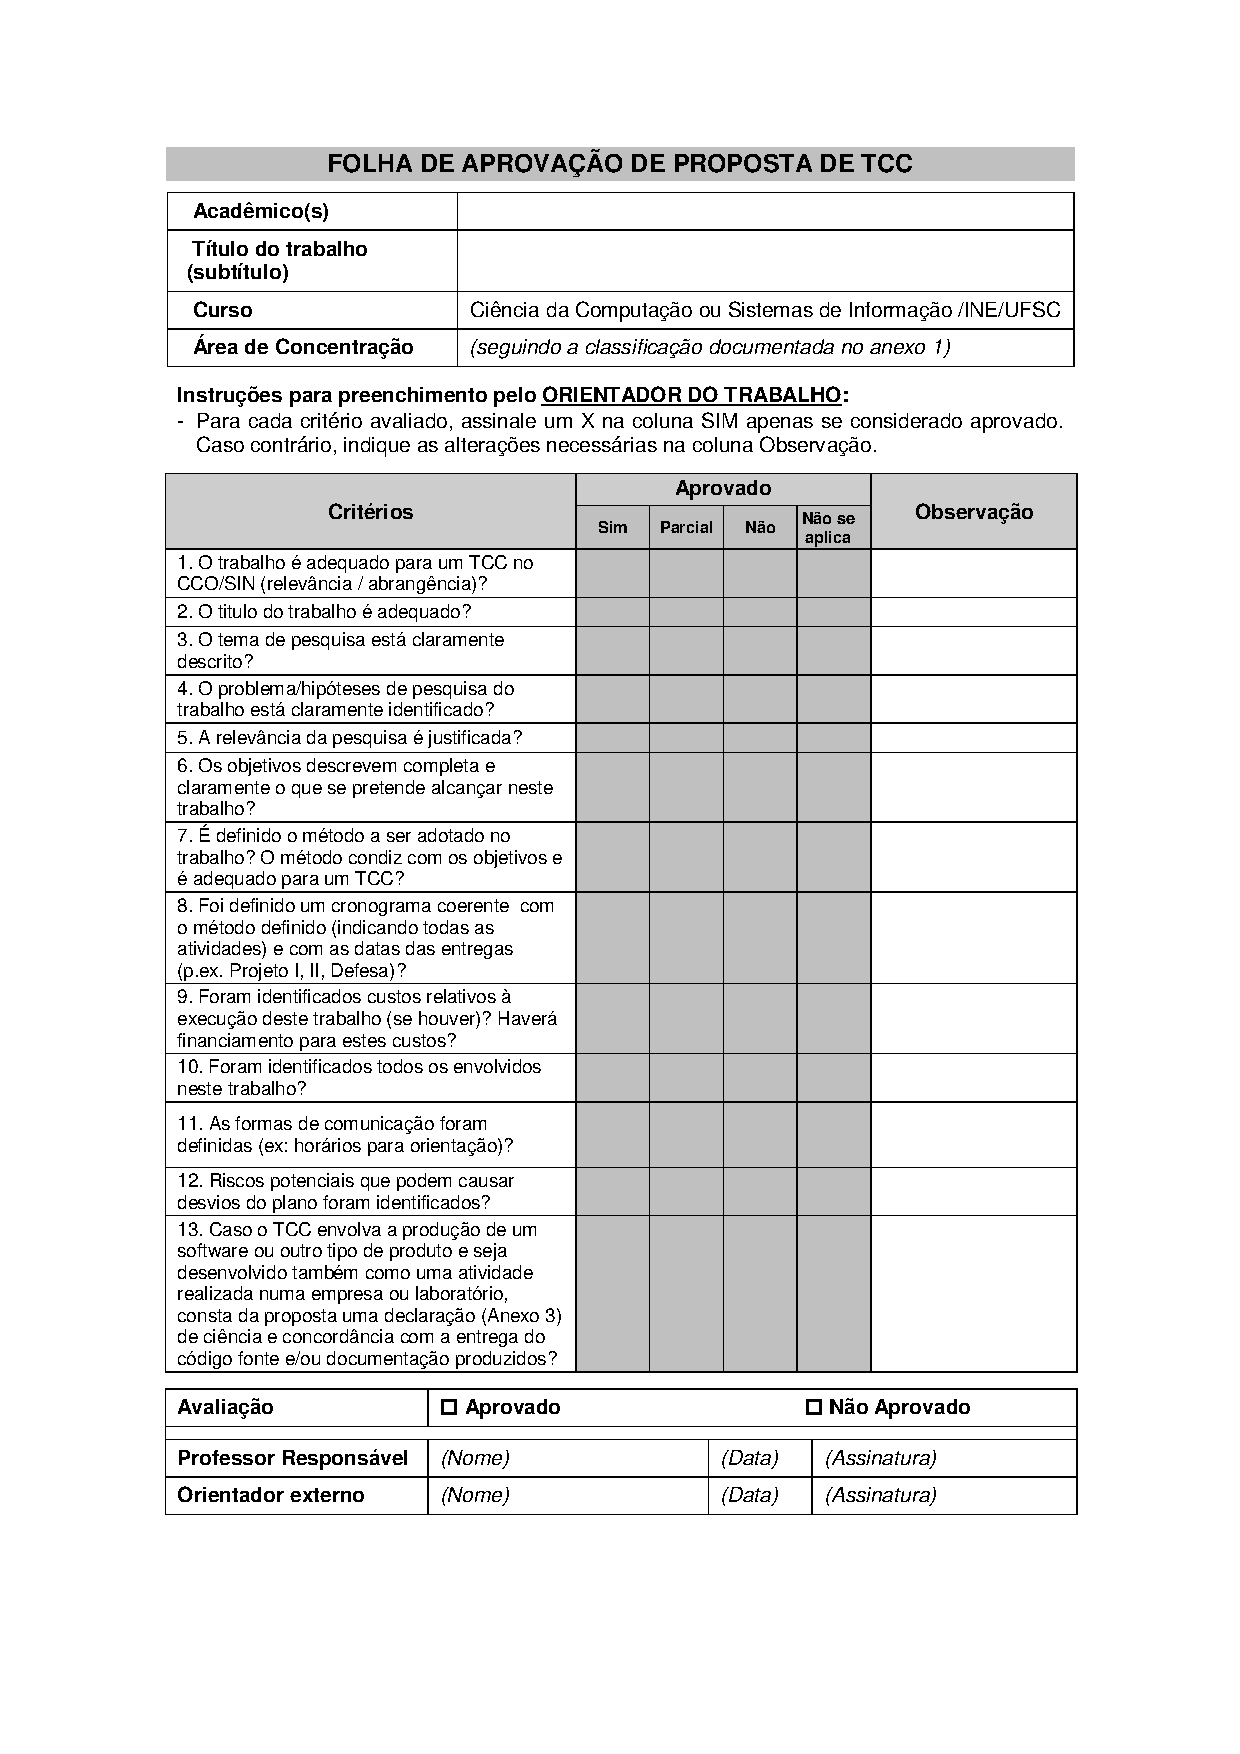
\includepdf{folha-de-aprovacao.pdf}
\end{folhadeaprovacao}

\begin{resumo}
Compiladores são os programas de computadores que fazem o papel de tradutor entre as linguagens de programação e as linguagens de maquina.
Eles recebem como entrada um texto escrito em uma linguagem fonte, chamado de programa fonte, e produzem como saída um texto escrito em uma linguagem de maquina alvo, chamado de programa alvo.
O processo de tradução executado por um compilador pode ser separado em duas grandes etapas: a etapa de analise e a etapa de síntese.
Entre elas existe uma linguagem intermediária.
O uso de uma linguagem intermediária é especialmente vantajoso pois, um compilador para a linguagem $i$ e maquina $j$ pode ser construído combinando um \textit{front end} para $i$ e um \textit{back end} para $j$.
O projeto LLVM é uma biblioteca de funcionalidades para otimização de código intermediário e geração de código alvo.
Estas funcionalidades são construídas ao redor de uma linguagem intermediária chamada \textit{LLVM intermediate representation}, ou LLVM IR\@.
O objetivo do trabalho consiste em propor o projeto de uma linguagem de programação similar a linguagem C e a confecção de seu compilador utilizando o ecossistema de ferramentas LLVM\@.
É esperada que a ferramenta consiga fazer a tradução de código fonte para código de maquina alvo e que o código de maquina alvo seja tão eficiente quanto ao gerado pela linguagem de programação C\@.

\vspace{\onelineskip}
\noindent
\textbf{Palavras-chave}: linguagem de programação\@. representação intermediária de código\@. compilador\@. LLVM\@. LLVM IR\@.

\end{resumo}

\begin{KeepFromToc}
  \tableofcontents
\end{KeepFromToc}

\textual{}

\chapter{Introdução}\label{cap:introducao}

Linguagens de programação são notações para descrever computações para pessoas e para máquinas.
Nos dias atuais todos os programas de computadores são descritos em alguma linguagem de programação
pois facilitam a comunicação das suas computações entre as pessoas que os desenvolvem.
Porém, antes que estas computações possam ser executadas por um computador,
elas necessitam ser traduzidas para uma linguagem de maquina passível de ser executada por um computador.

Compiladores são os programas de computadores que fazem o papel de tradutor entre as linguagens de programação e as linguagens de maquina.
Eles recebem como entrada um texto escrito em uma linguagem fonte, chamado de programa fonte, e produzem como saída um texto escrito em uma linguagem de maquina alvo, chamado de programa alvo.
Para que consigam realizar essa tradução, compiladores utilizam de modelos formais da teoria da computação e de teoria de linguagens formais.

O processo de tradução executado por um compilador pode ser separado em duas grandes etapas: a etapa de analise e a etapa de síntese.
Essas etapas podem ser mais uma vez subdivididas.

A etapa de analise, ou \textit{front end} de um compilador, pode ser subdividida em: analise léxica; analise sintática; analise semântica; e geração de código intermediário.
Além disso, a etapa de síntese, ou \textit{back end} de um compilador, pode ser subdividida em: otimização de código independente de maquina; geração de código alvo; e otimização de código dependente de maquina.

O uso de uma linguagem intermediária é especialmente vantajoso pois, um compilador para a linguagem $i$ e maquina $j$ pode ser construído combinando um \textit{front end} para $i$ e um \textit{back end} para $j$.
Assim, se desejarmos implementar $n$ linguagens de programação para $m$ maquinas, evitamos a construção de $n \times m$ compiladores construindo $n$ \textit{front ends} e $m$ \textit{back ends}.

A analise léxica consiste em identificar os lexemas presentes no código fonte e produzir \textit{tokens} para cada um dos lexemas encontrados.
Estruturas formais como expressões regulares e autómatos finitos, juntamente com um algorítimo de conversão~\cite{lesk1975lex}, podem ser utilizadas para geração automática de analisadores léxicos.

A analise sintática consiste em analisar os \textit{tokens} produzidos pelo analisador léxico de produzir uma arvore sintática.
Estruturas formais como linguagens livre de contexto e maquinas de pilha, juntamente com um algorítimo de \textit{parsing}~\cite{knuth1965translation}, podem ser utilizadas para geração automática de analisadores sintáticos.

A analise semântica consiste em analisar a arvore sintática produzida pelo analisador sintático e produzir código intermediário.
Estruturas formais como \textit{Syntax Directed Definitions} (SDD), juntamente a uma \textit{Syntax Directed Translation} (SDT), podem ser utilizadas para geração de código intermediário~\cite{Aho:2006:CPT:1177220}.

O \textit{back end} de um compilador realiza a etapa de síntese e é uma area muito importante de compiladores.
É o \textit{back end} que realiza as otimizações necessárias para que os programas de computador sejam eficientes.

O projeto LLVM~\cite{lattner2004llvm} é uma biblioteca de funcionalidades para otimização de código intermediário e geração de código alvo.
Estas funcionalidades são construídas ao redor de uma linguagem intermediária chamada \textit{LLVM intermediate representation}, ou LLVM IR\@.

Este trabalho tem como objetivo projetar uma linguagem de programação similar a C e desenvolver um \textit{front end} para a linguagem intermediária LLVM\@.
O mesmo vem a contribuir com a dissertação de mestrado do Evandro Chagas no PPGCC (Programa de Pós-Graduação em Ciência da Computação) UFSC, no qual há a especificação de uma linguagem de programação quântica.
Vale ressaltar que o escopo da presente proposta constitui da parte clássica~\footnote{O termo clássico é usado em contraponto ao termo quântico, ou seja, clássico é tudo que não é quântico.} da especificação dessa linguagem de programação quântica.

\chapter{Objetivos}\label{cap:objetivos}

O principal objetivo do trabalho proposto consiste em desenvolver uma linguagem de programação similar a linguagem C, usando o ecossistema LLVM para geração de linguagem intermediária.

\section{Objetivos específicos}

Os objetivos específicos são:
\begin{alineas}
  \item projetar uma linguagem de programação similar a C\@;
  \item implementar um analisador léxico, um analisador sintático e uma tradução dirigida a sintaxe;
  \item implementar uma ferramenta para controlar a otimização da linguagem intermediária LLVM\@. Além de controlar a tradução da mesma para código objeto;
  \item integrar a ferramenta ao processo de ligação de código do ambiente GNU/Linux;
  \item avaliar as decisões de projeto da linguagem de programação projetada quanto a linguagem C.
\end{alineas}

\chapter{Método de pesquisa}\label{cap:metodo_de_pesquisa}

Para atingir-se os objetivos específicos deste projeto serão seguidos os seguintes passos:
\begin{alineas}
  \item fundamentação teórica e estudos de artigos, livros, tendo como base o livro \textit{Compilers: Principles, Techniques, and Tools (2Nd Edition)}~\cite{Aho:2006:CPT:1177220}.
    Além de análise de tendencias em linguagens de programação existentes, de suas documentações e de suas implementações.
    Esta etapa esta prevista pelo cronograma na tabela~\ref{tab:cronograma} em \textit{Estudo da fundamentação teórica};
  \item projeto de uma linguagem de programação similar a C\@ e implementação de um compilador para a mesma.
    Esta etapa esta prevista pelo cronograma na tabela~\ref{tab:cronograma} em \textit{Desenvolvimento da solução};
  \item analise da linguagem de programação projetada e comparação com linguagens já existentes;
    Esta etapa esta prevista pelo cronograma na tabela~\ref{tab:cronograma} em \textit{Desenvolvimento da solução};
  \item desenvolvimento iterativo da monografia do trabalho de conclusão de curso.
    Incluindo entrega de um relatório parcial em Projeto I, uma entrega final e uma defesa publica.
    Esta etapa esta prevista pelo cronograma na tabela~\ref{tab:cronograma} em \textit{Desenvolvimento do relatório de Projeto I} e \textit{Desenvolvimento do rascunho do TCC}.
\end{alineas}

\chapter{Planejamento}

\section{Cronograma}\label{cap:cronograma}

O cronograma é descrito pela tabela~\ref{tab:cronograma}.

\begin{table}[h]
  \caption{Planejamento das etapas do trabalho de conclusão de curso}\label{tab:cronograma}
  \resizebox{\textwidth}{!}{
    \begin{tabular}{@{}lccccc@{}}
      \toprule
      \multicolumn{1}{c}{Etapas} & \multicolumn{5}{c}{Messes} \\
      \cmidrule(lr){2-6}
      & \multicolumn{2}{c}{2021} & \multicolumn{3}{c}{2022} \\
      \cmidrule(lr){2-3} \cmidrule(lr){4-6}
      & nov & dez & jan & fev & mar \\
      \midrule
      Entrega da ratificação de TCC
      &08&&&&\\
      Estudo da fundamentação teórica
      &\ding{55}&&&&\\
      Desenvolvimento da solução
      &\ding{55}&\ding{55}&\ding{55}&\\
      Redação do rascunho do TCC
      &\ding{55}&\ding{55}&\ding{55}&\ding{55}&\\
      Entrega do Rascunho do TCC
      &&&&23&\\
      Avaliação do Rascunho do TCC
      &&&&&3\\
      Defesa pública
      &&&&&$[3, 22]$\\
      Entrega do TCC
      &&&&&24\\
      \bottomrule
    \end{tabular}
  }
\end{table}

\section{Custos}\label{cap:custos}

Não há custos envolvidos.

\section{Recursos humanos}\label{cap:recursos_humanos}

O projeto sera orientado pelo professor Rafael de Santiago e coorientado pelo aluno de mestrado Evandro Chagas Ribeiro da Costa como indicado pela tabela~\ref{tab:envolvidos}.

\begin{table}[h]
  \caption{Envolvidos no projeto}\label{tab:envolvidos}
    \centering
      \begin{tabular}{@{}ll@{}}
        \toprule
        \multicolumn{1}{c}{Nome} & \multicolumn{1}{c}{Função} \\
        \midrule
        Rafael de Santiago & Responsável \\
        Rafael de Santiago & Orientador \\
        Evandro Chagas Ribeiro da Costa & Coorientador \\
        \bottomrule
      \end{tabular}
\end{table}

\section{Comunicação}\label{cap:comunicacao}

A comunicação sera efetuada através de reuniões intermitentes com o orientador e o coorientador.

\section{Riscos}\label{cap:riscos}

\begin{table}[h]
  \caption{Riscos do projeto}\label{tab:riscos}
    \resizebox{\textwidth}{!}{
      \begin{tabular}{@{}p{4cm}cccp{4cm}p{4cm}@{}}
        \toprule
        \multicolumn{1}{c}{Risco} & Probabilidade & Impacto & Prioridade & \multicolumn{1}{c}{Estratégia de resposta} & \multicolumn{1}{c}{Ações de prevenção} \\
        \midrule
        Perda de dados & baixa & alto & alta & Recuperação de versões anteriores & Utilizar serviços remotos de versionamento \\
        Negligenciar fator importante na especificação dos analisadores que é necessário para linguagem
        & médio & alto & alta & Refatoração da especificação dos analisadores & Analise continua das especificações utilizadas por outras linguagens \\
        \bottomrule
      \end{tabular}
    }
\end{table}

\postextual{}

\bibliography{bibliography.bib}

\end{document}
